\documentclass[a4paper]{article}
\usepackage{tabularx}
\usepackage{amsmath}
\usepackage{graphicx}
\usepackage{subcaption}
\usepackage{cite}

\usepackage[utf8]{inputenc}
\usepackage[T1]{fontenc}
\usepackage{float}
\usepackage{multirow}
\usepackage{listings}

\usepackage{indentfirst}
\usepackage{tensor}
\usepackage{amssymb}
\allowdisplaybreaks
\usepackage{bm}
\newcommand{\at}[2][]{#1|_{#2}}
\newcommand\numberthis{\addtocounter{equation}{1}\tag{\theequation}}
\newcommand\norm[1]{\left\lVert#1\right\rVert}
\usepackage{caption}
\captionsetup[lstlisting]{font={small}}
\captionsetup[figure]{font=small}
\captionsetup[table]{font=small}
\usepackage{breqn}

\begin{document}

\title{Report of the CryptoNets Project}

\makeatletter
\let\thetitle\@title
\let\theauthor\@author
\let\thedate\@date
\makeatother

\begin{titlepage}
	\centering
    \vspace*{0.5 cm}
    
\includegraphics[scale = 0.75]{images/SapienzaLogo}\\[1.0 cm]	% University Logo
    \vspace*{-0.3cm}
    \textsc{\large Ingegneria Informatica, Automatica e Gestionale}\\[2.0 cm]	% Department Name
    \vspace*{1.2cm}
    { \fontsize{20.74pt}{18.5pt}\selectfont\bfseries \thetitle \par } % title
    \vspace*{0.1cm}
    \textsc{\Large Neural Networks}\\[0.5 cm] % course name
    \vspace*{5.6cm}
	\begin{minipage}{0.4\textwidth}
		\begin{flushleft} \large
			\emph{Professor:}\\
			Aurelio Uncini\\
		\end{flushleft}
	\end{minipage}~
	\begin{minipage}{0.4\textwidth}
		\begin{flushright} \large
			\emph{Students:} \\
            Armando Nania\\
            Josè Luis Bustamante
		\end{flushright}
	\end{minipage}\\[2 cm]
\end{titlepage}


\tableofcontents
\newpage

\section{Introduction}

The two fields of "cryptography" and "machine learning" studies have produced great results in recent years. Neural networks (a specific class of machine learning algorithms) have reached levels of accuracy never obtained with other methods in tasks such as image classification and speech recognition. On the other hand, cryptography research has produced a new set of cryptographic scheme that preserve most of the interesting statistical structure of the data \cite{safeai}. These schemes are called homomorphic encryption: they were first proposed in 1978 \cite{firstHomEnc}, and the first Fully Homomorphic algorithm was found in 2009 \cite{10.1007/978-3-642-29011-4_28}. Since then other algorithms have been discovered that allow greater speed by sacrificing part of the flexibility of the cryptographic scheme, and now the intersection between these two research field (homomorphic algorithms and deep learning) is revolutionizing the world of cloud computing. The use of this technology has advantages: for example, an encrypted neural network is protected from those who might want to steal it. It allows the decentralization of the AI, making it possible to be trained in insecure environments without risk by the owner of the network. Moreover, many people are frightened by the possibility that an artificial superintelligence can harm humanity. Some experts, like Stephen Hawking, Elon Musk and others have signed an open letter that focuses on these issues, calling for greater responsibility during the development of artificial intelligence \cite{open-letter}. The application of cryptography to neural networks can represent a potential technical solution to this problem: if the AI is encrypted, then from its point of view the whole external world is encrypted. So the human who has the key to decipher the neural network has control over his intelligence: he can decrypt individual predictions that it makes, without having to decrypt the network itself \cite{safeai}. But the main application addressed by this project is Data Privacy. Progress in fields such as stock market efficiency is hampered by the lack of open participations, due to the privacy of datasets. In fact, most stock market data are not publicly available, because it would be an economic loss to disclose them, so the owners usually keep them private. Using cryptography, however, it is possible to publish a datasets for training a model without giving away valuable data \cite{numerai}. Beside training, cryptography is also useful during the inference stage. Take for example a hospital that would like to use a cloud service to predict the probability of readmission of a patient within the next 30 days. In order to use this service without violating the ethical and legal requirements regarding the confidentiality of patient information, the hospital can take advantage of CryptoNet, the algorithm described in this report.

\subsection{Roadmap}

In this report we will analyze the work that we done on the CryptoNets. The project is based on \cite{dowlin2016cryptonets}, developed by Microsoft researchers. The report is structured as follows: in Section 2 we analyze how the cryptographic algorithm works. In Section 3 we give a description of the neural network and of some problems arising in the use of the cryptographic scheme. In Section 4 we introduce the Microsoft software SEAL library used in this project and to follow, in Section 5, we describe the rest of the code developed. The report closes with the presentation of the results obtained in Section 6 and the conclusion in Section 7.

\section{Homomorphic Encryption}

Cryptography is the practice and study of techniques for secure communication in the presence of third parties called adversaries. In its simplest form it is made up of a cryptographic function $f(\cdot)$, that can be inverted but only if you have the right key. Therefore, using a correct pair of public and secret keys, we have that $f^{-1}(f(n))=n$ for each n on which $f(\cdot)$ is defined. Traditional cryptography does not allow any operation to be performed on the encrypted data $f(n)$, otherwise you lose the original information. Homomorphic cryptography, on the other hand, is able to preserve both the additive and multiplicative structure of the integers. That is, given two integers $a$ and $b$, the following equations are valid:

\begin{align*}
  f^{-1}(f(a)+f(b)) &= a+b\\
  f^{-1}(f(a)*f(b)) &= a*b
\end{align*}

The use of these two operations, sum and product, allows us to make encrypted predictions starting from the encrypted data in input.

\subsection{The FV algorithm}

The algorithm described in the paper and used in the original CryptoNets project is YASHE, contained in the software library called SEAL \cite{dowlin2016cryptonets}. But in the meantime the library has been updated. The version that we use is v2.3, in which the algorithm implemented is a variant of the Fan-Vercauteren (FV) scheme \cite{seal-manual}. Here we present the basic version of the FV algorithm, and then we will discuss the particular version coded inside the SEAL library.

The FV scheme is an isomorphism between polynomial rings. A polynomial ring $R^a_b$ is the space consisting of all polynomials reduced modulo $x^a+1$, where the coefficients are reduced modulo $b$, ie $R^a_b = \mathbb{Z}_b[x]/(x^a+1)$. In particular, the scheme takes the polynomials from the ring $R^n_t$ as input and transforms them into an array of polynomials, each of them belonging to $R^n_q$. The polynomial array has a minimum size of 2, but increases each time a homomorphic multiplication is performed. It is possible however to subsequently reduce the size of the array (up to a minimum of 2) using a process called relinearization.

The algorithm randomly generates the polynomial $s$ in $R^n_2$: it constitutes the private (or secret) key. We will denote by $a \leftarrow R^b_c$ that $a$ has been generated with a uniform distribution from the polynomial ring $R^b_c$, and with $a \leftarrow X$ that a has been generated with a truncated Gaussian distribution in the space $X$, so $s \leftarrow R^n_2$. The public key is the array $(\text{p}[0], \text{p}[1]) = ([-(as + e)]_q, a)$, with $a \leftarrow R^n_q$, and $e \leftarrow X$. The cryptographic scheme provides also the use of some special keys, called evaluation keys, to carry out the relinearization operation. The number of evaluation keys is equal to $l + 1$, with $l=\lfloor \log_w q \rfloor$ and $w$ parameter of the algorithm. Each evaluation key is composed of an array of two elements, so the $i$-th key is given by: $\text{evk}[i] = ([-(a_is+e_i)+w^is^2]_q, a_i)$, where $a_i \leftarrow R^n_q$, $e_i \leftarrow X$.

A message m $\in R^n_t$ is encrypted by computing

\begin{equation*}
    \text{c} = \left(\left[\left \lfloor \frac{q}{t} \right \rfloor m + \text{p}[0] u + e_1 \right]_q , [\text{p}[1] u + e_2 ]_q\right) 
\end{equation*}

\noindent where $u \leftarrow R^n_2$, and $e_1, e_2 \leftarrow X$. Decrypting is done by computing

\begin{equation*}
    \text{m} = \left[\left\lfloor  \frac{t}{q}  [\text{c}[0] + \text{c}[1] s]_q  \right\rceil\right]_t
\end{equation*}

Two ciphertexts $\text{c}_1$ and $\text{c}_2$ can be added together in $R^n_q$ like this:

\begin{equation*}
    \text{c}'=(\text{c}_1[0] + \text{c}_2[0], \text{c}_1[1] + \text{c}_2[1])
\end{equation*}

Multiplication is more complicated. First we calculate a new array of 3 elements like this:

\begin{align*}
    &\text{c}[0] = \left[\left\lfloor\frac{t}{q}\text{c}_1[0]\text{c}_2[0]\right\rceil\right]_q\\
    &\text{c}[1] = \left[\left\lfloor\frac{t}{q}(\text{c}_1[0]\text{c}_2[1]+\text{c}_1[1]\text{c}_2[0])\right\rceil\right]_q\\
    &\text{c}[2] = \left[\left\lfloor\frac{t}{q}\text{c}_1[1]\text{c}_2[1]\right\rceil\right]_q
\end{align*}

Then the relinearization process is performed:

\begin{align*}
    &\text{c}'[0] = \text{c}[0]+\sum\limits_{i=0}^l\text{evk}[i][0](\text{c}[2])^{(i)}\\
    &\text{c}'[1] = \text{c}[1]+\sum\limits_{i=0}^l\text{evk}[i][1](\text{c}[2])^{(i)}
\end{align*}

For more details on the FV algorithm, it is possible to consult \cite{Fan2012SomewhatPF}.

\subsection{Mismatch between data type}

As is evident at first sight, there is a problem of incompatibility between the type of data processed by a neural network and the type of data processed by the homomorphic algorithm. The first of them works with floating-point numbers, while the second one is basically a transformations between polynomials. Before seeing how the neural network works, we must therefore discuss the encoding we shall use. The SEAL library already offers the possibility of transforming a real number into a polynomial, but this method is very inefficient, because much of the polynomial is wasted. As we will see later, the Chinese remainder theorem applied to the polynomials allows us to encode in a single polynomial several different integers, which will be manipulated in parallel and all in the same way. This allows us to use less polynomials in total, and to make computation faster. The idea is therefore to use a polynomial of degree $n$ to encode $n$ values, where each value is taken from a different input, but relative to the same position in the data input structure. For example we construct the polynomial "first pixels" using the values taken from the first pixel of each of the $n$ images. Then we do the same for the "second pixels" polynomial, the "third pixels" polynomial, and so on, until all the input data have been encoded. This technique is called CRT batching. It is therefore necessary that the data to be transformed into polynomials are integers modulo $t$. To do this it is possible to perform a pre-encoding phase, in which the data are multiplied by a constant (that we call precision), rounded and reduced modulo $t$. It is also necessary to carry out the same procedure on the weights of the neural network (more details on this will be presented in the Section 3.3). The precision parameter chosen to multiply the data affects the entire computation. There is a trade-off between the accuracy of the transformed neural network, and the chosen size of the parameter $t$. $t$ in turn has a trade-off: it must be large enough so that during the entire calculation process no number exceeds $t/2$ (see the Section 2.4: Negative numbers). But at the same time a larger $t$ implies more noise in the cryptography algorithm. In our project we chose $\text{precision} = 100$; in this way all the numbers computed are smaller than $2^{80}$, which guide us in selecting the parameters for the encryption scheme. But a choice of t such that $t>2^{80}$ makes the homomorphic algorithm unusable, unless the Chinese remainder theorem is used again, but this time for a different purpose: to factorize $t$.

\subsection{Chinese remainder theorem}

The Chinese remainder theorem is a mathematical theorem dating back to the 3rd century CE, and is widely used in the field of cryptography. It allows to break down a number into a set of smaller numbers, and to reconstruct the original number starting from that set. Moreover it allows to operate on the set of small numbers, preserving the sum and product operations, just like the homomorphic schemes. The formulation is the following: given $k$ pairwise coprime numbers $n_1, n_2, ..., n_k$, we can break down a number $x$ like this:

\begin{align*}
    &x = a_1 & (\text{mod }n_1)\\
    &x = a_2 & (\text{mod }n_2)\\
    &...\\
    &x = a_k & (\text{mod }n_k)
\end{align*}

The numbers thus obtained $a_1, a_2, ..., a_k$ can be used, together with the $k$ coprime numbers, to reconstruct the number $x$, provided that $x\in[0,N)$, where $N=n_1n_2...n_k$. To do this, we must first compute the coefficients of Bézout's identity, $r_i$ and $s_i$, such that

\begin{align*}
    r_in_i+s_i\left(\frac{N}{n_i}\right) = \text{gcd}\left(n_i, \left(\frac{N}{n_i}\right)\right) = 1 && \text{for }i=1,2,...,k
\end{align*}


\noindent where gcd is the greatest common divisor, which is equal to 1 since $n_i$ and $N/n_i$ are coprime. To do this it is possible to use the Extended Euclidean algorithm. After that, it is possible to reconstruct the starting number in this way:

\begin{align*}
    & x = \sum\limits_{i=1}^k a_i s_i \frac{N}{n_i} & (\text{mod }N)
\end{align*}

This result is very useful, if not indispensable, in this project. In the original paper, which uses the old version of SEAL, the Chinese remainder theorem is used twice for two purposes: to break down the parameter $t$, and to unify more data into a single polynomial. With "break down the parameter $t$" we means to choose a set of numbers $t_i$ such that their multiplication gives the desired $t$. Therefore, in the above diagram, $t$ corresponds to the parameter $N$, and $t_i$ corresponds to $n_i$. It is important to remember that the individual $t_i$ chosen must be pairwise coprime. This is assured since in order to use CRT batching there is a more stringent requirement on the choice of parameters $t_i$: they must be prime numbers and equal to 1 (mod $2n$). If this requirement is satisfied, then there exists an $\zeta \in \mathbb{Z}_{t_i}$ so that we can break down the polynomial $x^n+1$ as follows:

\begin{align*}
    &x^n+1 = (x - \zeta)(x - \zeta^3)...(x - \zeta^{2n-1}) & (\text{mod }t_i)
\end{align*}

Therefore it is possible to decompose the polynomial ring $R^n_{t_i}$ into $n$ spaces $\mathbb{Z}_{t_i}$:

\begin{equation*}
    R_{t_i} \cong \prod \limits_{i=0}^{n-1} \mathbb{Z}_{t_i}
\end{equation*}

This is the procedure underlying CRT batching. More details are shown in \cite{seal-manual}.

As we mentioned before, the version of SEAL used in our project is v2.3, which uses a variant of the FV algorithm described above. In particular, in our version of the software library the theorem is used on three occasions, two of which correspond to those of the original paper, described above. The third and new use of the theorem lies in the decomposition of the parameter $q$ into smaller numbers. Also in this case we mean to break down the parameter $q$ with a set of numbers $q_i$ such that $q_1q_2...q_i = q$. This is a variant of the cryptographic scheme which is not present in the original FV algorithm \cite{Fan2012SomewhatPF}. Due to this fact, the parameter $q$ differs between the two SEAL versions. In the original CryptoNets project, the researchers used 192 bits to represent $q$. We instead use 4 numbers, all between 55 and 60 bits, whose product gives a 230 bit number. So our project has a slightly larger $q$
, which slightly decreases the noise produced by the cryptographic algorithm.

\subsection{Negative numbers}

A final consideration concerning the use of the cryptographic scheme is given by the problem of negative numbers. The data manipulated by the neural network are always reduced modulo $t$, even when they are encrypted. Which means that at any time of the computation in the neural network, if you decrypt the output of a layer and recompose its values with the inverse of CRT batching, each resulting number will be an integer between 0 and $t$ ($t$ excluded). This can be a problem, as the original neural network, in addition to presenting floating-point numbers, also manipulate negative numbers. It can happen, in fact, that in the final layer there are negative numbers which, once reduced modulo $t$, become positive. Because now they're positive, these numbers can influence the choice of the final class for a certain input. In fact, at the end of the neural network computation, the prediction is given by choosing the class associated with the highest value among those present in the output neurons. It is therefore possible that one of those values which, in the original neural network, would have been negative and not chosen, is chosen. To avoid this problem, we need to find a way to encode negative numbers within the space of integers $[0, t)$. To do this, we use the following scheme:

\begin{figure}[H]
	\centering
	\makebox[\columnwidth]{
		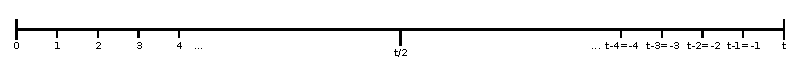
\includegraphics[width=0.8\paperwidth]{images/fig1.pdf}
	}
    \caption{Encoding of negative numbers in the $[0,t)$ span.}
    \label{fig:im1}
\end{figure}

\noindent so we divide the set $[0, t)$ into two parts: the first part contains only the positive numbers, while the second part contains only negative numbers. This is because given a negative number $-n$, its reduction modulo $t$ is equal to $t-n$. To do this, and to avoid that the two sub-sets overlap, it is therefore mandatory that no number during the computation of the neural network, taken as an absolute value, exceeds half of $t$: $\forall  n, |n|<t/2$. This allows us to reconstruct the output, after using the Chinese remainder theorem, using the following algorithm:

\lstset{frame=tb,
  language=Python,
  breaklines=true,
  showstringspaces=false,
  columns=flexible,
  numbers=none,
  tabsize=3,
  escapeinside={(*@}{@*)}
}

\begin{lstlisting}[frame=single]
n = crt_inverse(array)
negative_threshold = t / 2
if n > negative_threshold:
    n = n (*@-@*) t
\end{lstlisting}

\clearpage

\section{Neural Network}

The CryptoNet project can be summarized in this graph:

\begin{figure}[H]
	\centering
	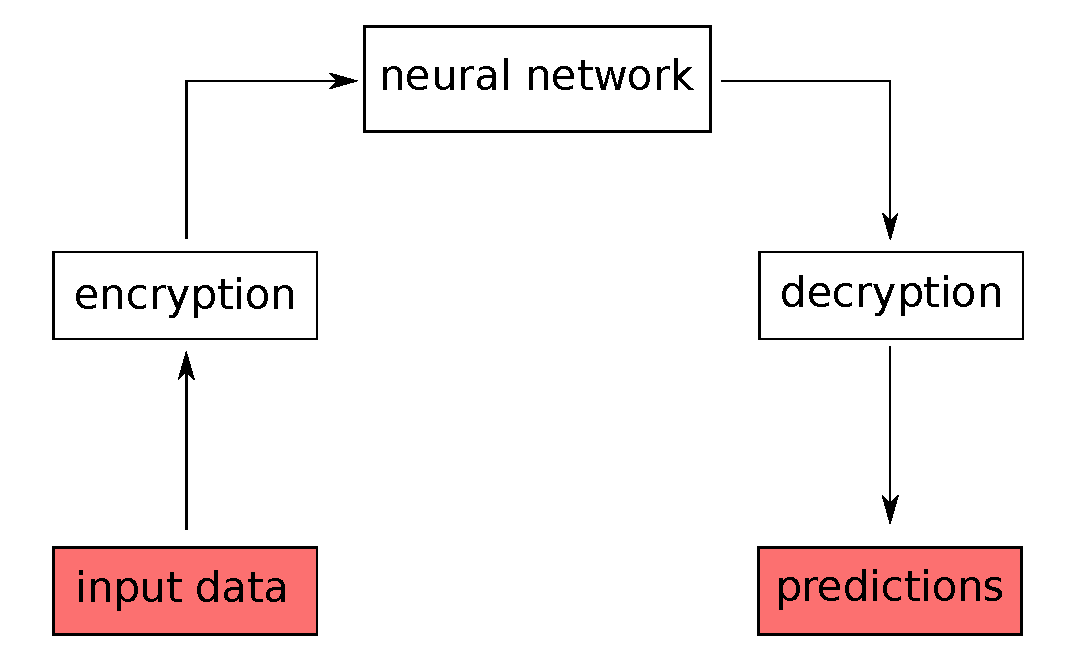
\includegraphics[width=0.8\textwidth]{images/fig2.pdf}
    \caption{The CryptoNets scheme.}
    \label{fig:im2}
\end{figure}

\noindent that is, it is a matter of applying a neural network to encrypted data to obtain encrypted predictions, and finally decrypt these to classify the initial input (image classification). But as we'll show, this scheme involves a simplification, ie it does not consider the process followed to obtain a model that can be applied to encrypted data. Below, we will analyze the problems that arise in the use of homomorphic cryptography techniques on neural networks, as well as other considerations regarding the network.

\subsection{The fundamental operations}

As we have shown in the Section 2, the only operations allowed by the homomorphic algorithm are the sum and the product. This partially limits the operations that can be performed by the network. Furthermore, it is important to remember that we are dealing with polynomials. In particular, in a neural network, a single neuron corresponds to the application of an activation function to the weighted sum of the outputs from neurons in the previous layer, to which is added a weight called bias:

\begin{equation*}
    y = f\left(\sum\limits_i w_i x_i + b\right)
\end{equation*}

\noindent with $x_i$ the previous outputs, $w_i$ the weights and $b$ the bias. But as said, the data to be manipulated are polynomials, and not simple scalar numbers. This means that we must consider every $x_i$ not as a single number, but as a polynomial, whose coefficients come from values of different images. So we can identify in the previous equation four different operations: the polynomial-scalar product, given by the multiplication of $x_i$ with $w_i$; the polynomial-polynomial sum, given by the sum of the single weighted polynomials; the polynomial-scalar sum, given by the sum of the resulting polynomial with the bias; and the activation function. The first two operations are straightforward, and they are obtained without the use of particular artifices (apart the reduction modulo $q$ of the coefficients). The polynomial-scalar product occurs simply by multiplying each of the single coefficients by the parameter $w_i$:

\begin{align*}
    &w_i(a_0+a_1x+a_2x^2+...+a_{n-1}x^{n-1}) =\\
    &\quad = w_ia_0+w_ia_1x+w_ia_2x^2+...+w_ia_{n-1}x^{n-1}
\end{align*}


This allows us, during the computation of the neural network, to momentarily neglect the fact that they are polynomials, and to treat each coefficient separately from the other, as in a normal neural network. The same applies to the polynomial-polynomial sum:

\begin{align*}
    &(a_0+a_1x+...+a_{n-1}x^{n-1})+(b_0+b_1x+...+b_{n-1}x^{n-1}) =\\
    &\quad = (a_0+b_0)+(a_1+b_1)x+...+(a_{n-1}+b_{n-1})x^{n-1}
\end{align*}


The polynomial-scalar sum is more complicated. What we want to obtain is that every value included in the polynomial is treated in the same way, ie we would like to obtain an output given by the sum of the input polynomial and of another virtual polynomial constructed using the bias $b$ for all coefficients:

\begin{equation*}
    b+bx+bx^2+...+bx^{n-1}
\end{equation*}

But adding this polynomial would not give the desired result. This is due to the type of encoding used, ie CRT batching. In particular, this type of encoding spreads the information of the various inputs on all the coefficients. That is, given the polynomial $(a_0 + a_1x + ... + a_{n-1}x^{n-1})$, $a_0$ does not correspond to the value of the pixel taken from the first image and $a_1$ does not correspond to the value of the pixel taken from the second image. Rather, $a_0$ contains part of the pixel values of all images, which is the quantity to be added to each coefficient during decoding. What we need to do is, therefore, encode an array so constructed: $\left[ \begin{matrix}b&b&...&b\end{matrix} \right]$ with CRT batching and use the resulting polynomial during computation in the neural network. The polynomial that is obtained in this way is the following:

\begin{equation*}
    (b+0x+0x^2+...+0x^{n-1})=b
\end{equation*}

So we just add b to the first position of the input polynomial:

\begin{align*}
    &(a_0+a_1x+...+a_{n-1}x^{n-1})+b =\\
    &\quad = (a_0+b)+a_1x+...+a_{n-1}x^{n-1}
\end{align*}

The activation function deserves particular attention. Typical functions, such as the sigmoid and the ReLU, are non-polynomial functions. The approach taken by us in this project is the same as the one followed in the original paper: we use the lowest-degree non-linear polynomial function, which is the square function: $\text{sqr}(z)=z^2$. But, as before, this does not mean to square each of the coefficients of the polynomial. To square a polynomial it is necessary to follow the procedure described in the Section 2.1. This operation is managed by the SEAL library, and is the only operation for which the software library is used directly.

\subsection{Scaling the weights}

Another problem for the design of the neural network concerns the values of the weights. As already mentioned, homomorphic cryptography works with polynomials whose coefficients are integers modulo $t_i$ (see the Section 2.3 to understand why the index $i$). If we use real numbers for the weights in the model, then the result of the operations would be polynomials whose coefficients are no longer integers, which would completely destroy the predictions. To avoid this it is necessary to scale the weights of the network, just like with the data: multiplication by a constant (called precision), rounding and reduction modulo $t_i$. The reduction modulo $t_i$ is necessary so that it is possible to use the Chinese remainder theorem during the encoding of large numbers. Moreover, this will prevent the weights from being negative, thus avoiding multiplying a negative parameter of the network with a positive input, that is, avoiding negative numbers in output that would prevent the decoding of the polynomials (more information in the Section 2.4: Negative numbers).

\subsection{Plain operations}

The last point to consider is that the previous points are valid only with plain polynomials. In order to operate in the encrypted polynomials ring, the most intuitive way is to first encrypt the constants and then perform the addition or multiplication operation. However, this process is both computationally intensive and adds a large amount of noise if the operations are multiplications. Furthermore, the process would force the cloud service to provide the customer with its own neural network, so that the latter can encrypt it and send it back to the cloud (since it is necessary that weights and data are encrypted with the same key). In addition to being very inefficient, this procedure forces the cloud to give away valuable information such as the neural network weights. A more efficient way is to perform operations with plain weights. Let $\text{c}=([\lfloor q/t\rfloor m+\text{p}[0]u+e_1]_q,[\text{p}[1]u+e_2]_q)$ be the encrypted message and $b$ the known constant. Addition can be achieved by multiplying $b$ by $\lfloor q/t\rfloor$ and adding that to the first element of c:

\begin{equation*}
    \text{c} = \left(\left[\left \lfloor \frac{q}{t} \right \rfloor (m+b) + \text{p}[0] u + e_1 \right]_q , [\text{p}[1] u + e_2 ]_q\right) 
\end{equation*}

This is essentially just encrypting $b$ with no noise and performing normal homomorphic addition. For multiplication, even the scaling is not needed since:

\begin{equation*}
    \text{c}w = \left(\left[\left\lfloor\frac{q}{t}\right\rfloor(mw)+\text{p}[0]u'+e'_1\right]_q,[\text{p}[1]u'+e'_2]_q\right) 
\end{equation*}


This is very efficient, and allows the machine learning service provider to keep the neural network secret. However, it's worth remembering, in the case of the plain sum, to add the scaled parameter $b$ only to the first coefficient of the polynomial, as already explained in the Section 3.1: The fundamental operations.

\subsection{Network architecture}

The architecture of the network is very simple, and corresponds to the simplified version of the original paper \cite{dowlin2016cryptonets}. It consists of 5 layers. In order they are: the convolution layer, the first square layer, the pool layer, the second square layer, the output layer.

The convolution layer takes images with 28x28 pixel as input. However, since large numbers have been coded using the crt technique, each number has been decomposed into 5 numbers. Therefore the input tensor has dimension equal to $n$x28x28x5, where $n$ is the number of inputs of which we want to infer predictions. For each example, on each of the 5 images per example, a convolution is applied with a 5x5 kernel, stride (2, 2), and mapcount 5. The output should therefore be a $n$x5x13x13x5 tensor but, since it also executes the flattening operation simultaneously, has in fact size $n$x845x5. The first square layer uses the SEAL library to perform omomorphic multiplication with subsequent relinearization. The output therefore again has size $n$x845x5. The pool layer is actually a fully connected layer, in which we pass from 845 neurons (by image and by element in the sequence crt) to 100, so the output becomes $n$x100x5. The second square layer works like the first, and the last layer, the output layer, goes from 100 neurons to the 10 neurons of the image classes, so the final output of the model is $n$x10x5. The result must then be first decrypted, then decoded, and finally reconstructed as in the Section 2.3. At this point the predictions are computed for each of the $n$ inputs using the argmax function.

\subsection{Training}

As explained in \cite{dowlin2016cryptonets}, this project is entirely focused on the inference phase, so we make the assumption that the cloud already has a model. In our case, as in the original project case, it would be a neural network that was previously trained using a set of unencrypted data. We used the gradient descent method, with a learning rate of 0.001, batch size of 100 and 50 training epochs. The dataset is divided into a training set of 55,000 pairs of image-predictions, and another 10,000 pairs in the test set. The accuracy achieved in this phase, without applying any of the previously described techniques, is 98.43\% (more on this in the Section 6: Results).

\clearpage

\section{SEAL library}

The SEAL library is a C++, open source cryptographic software library, developed by Microsoft. It's the tool we used in our project to code, cipher, decrypt and decode the data to be manipulated. We also used the library for the activation function layers in the neural network. In this section we will show in detail the wrapper we created to invoke the SEAL functions from python.

\subsection{The encrypted polynomials ring}

As we have already mentioned in the cryptography section, SEAL does not directly implement the FV scheme, but instead makes some changes to this homeomorphic algorithm. In particular, as we have already seen, the Chinese remainder theorem is used to break down the parameter $q$ into various divisors $q_i$, all with a maximum of 60 bits. Moreover, an encrypted message is not an array of polynomials in $R^n_q$, is actually an array of polynomials in $R^{n+1}_q$. It is important to keep this point in mind while programming the operations: for example, the polynomial-scalar sum must be performed once every $n+1$ coefficients, for each $q_i$ of the first size. An encrypted message, in fact, is formed as follows:

\begin{figure}[H]
	\centering
	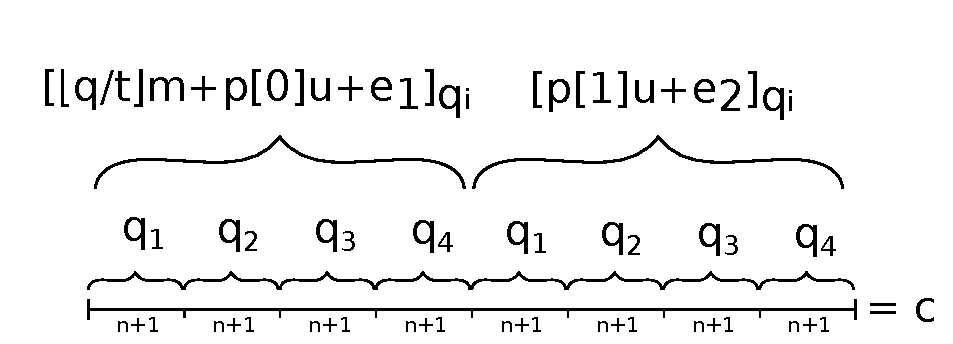
\includegraphics[width=\textwidth]{images/fig3.pdf}
    \caption{The encrypted message scheme.}
    \label{fig:im3}
\end{figure}

In this example we have a module $q$ composed of four divisors ($q1$, $q2$, $q3$, $q4$), and the encrypted message has size equal to 2. Therefore we have a total of 8 polynomials, and each polynomial has degree $n$, for a total of $(n+1)\cdot8$ coefficients. This is the minimum number of coefficients needed to encode $n$ values of the input data. Of the 8 polynomials, the first four contain the original information $(\lfloor q/t \rfloor m)$, the other four contain instead only information on the added noise, so that, together with the secret key, the message can be decrypted. The coefficients of the eight polynomials are reduced modulo $q_i$, with $i$ based on the position of the polynomial. In particular they are repeated: $i = 1,2,3,4$ for the first half, and again $i = 1,2,3,4$ for the second half. All this must be taken into account when programming the neural network. (see the Section 3: Neural network).

\subsection{The wrapper}

The wrapper for the SEAL library consists of two parts: a \texttt{wrapper.cpp} file and a \texttt{wrapper.py} file. We first introduce the C++ part, and then we'll show the Python part.

\subsubsection{The C++ wrapper}

The \texttt{wrapper.cpp} file declares all the functions that must be used in the project. They are:


\lstset{frame=tb,
  language=C++,
  breaklines=true,
  showstringspaces=false,
  columns=flexible,
  numbers=none,
  commentstyle=\color{dkgreen},
  stringstyle=\color{mauve},
  tabsize=3,
  morekeywords={uint64_t}
}
\begin{lstlisting}[frame=single]
void generate_new_keys()
void initialize()
void deallocate()
void encrypt_tensor(uint64_t *input, uint64_t *output, int input_axis0_size, int data_size)
void decrypt_tensor(uint64_t *input, uint64_t *output, int output_axis0_size, int data_size)
void square_tensor(uint64_t *input, uint64_t *output, int input_axis0_size, int data_size)
\end{lstlisting}

The first function generate a new set of keys for the encryption system, and save them in the folder "keys". The initialize() function loads the those keys in memory to be used; the deallocate() function does the opposite, that is it frees the memory used by the keys and the SEAL library. The three following functions correspond to the three basic operations of encrypting, decrypting and squaring. The important thing to note here is that they take as input an entire tensor, which, in the case of decrypt_tensor($\cdot$) and square_tensor($\cdot$), is a set of encrypted polynomials. encrypt_tensor($\cdot$) instead takes as input a data tensor and converts it into an encrypted polynomial tensor, ie it deals with both CRT batching and actual encryption. Similarly, decrypt_tensor($\cdot$), after decrypting the polynomial tensor, decodes it. The exact number of messages encrypted in output to the encrypt_tensor function depends on the number of images we want to transform, namely input_axis0_size, and the size of each image: data_size. A polynomial of $n$ coefficients can encode up to $n$ values of different images, therefore the number of messages encrypted in output to the function is equal to $\lceil \text{input_axis0_size}/n\rceil\cdot\text{data_size}\cdot5$, where 5 is the number of factors $t_i$ of the $t$ chosen.

\subsubsection{The Python wrapper}

The python part of the wrapper uses ctypes, the Python module, to call the dynamic library compiled by the \texttt{wrapper.cpp} file. It takes care of adapting the data in the useful form to the library in C ++. For example, it takes care of flattening the tensors before passing them as parameters to the function to call, or it calculates the data_size parameter. It has two special methods, __init__() and __del__(), of which the first deals with loading all the necessary data into memory, such as the parameters $n$, $t$, $q$, $k$, and the dynamic library libseal.so, and the second deallocates the library from the ram, freeing the memory from previously loaded data.

\subsection{The selected parameters for the cryptography scheme}

As discussed above, one of the differences between the SEAL version used in \cite{dowlin2016cryptonets} and that we use is the need, in our case, to break down the parameter $q$ into several divisors. This prevents us from using the same identical parameters used by that paper, since the numbers chosen for the parameter $q$ in the original project are prime numbers. We have therefore decided to keep the choices of the other two parameters ($n$ and $t$) identical and to change only $q$. It is important to note that, due to the decomposition of the $t$ parameter, these parameters are not part of a single encryption scheme, but rather there are 5 schemes: one for each $t_i$. So for each $t_i$ we decided to keep the number of coefficients $n$ (as in \cite{dowlin2016cryptonets}), and the parameters $q$ (differently from how it was done in the original project). Therefore, the five schemes are:

\begin{center}
\begin{tabular}{ |c|P{2cm}|P{2cm}|c| } 
\hline
Scheme number & n & t & q \\
\hline
\hline
& & & \\
\multirow{4}{*}{\#1} & \multirow{4}{*}{4096} & \multirow{4}{*}{40961} & 36028797014376449 \\
& & & 36028797013327873 \\
& & & 1152921504241942529 \\
& & & 1152921504369344513 \\
& & & \\
\hline
& & & \\
\multirow{4}{*}{\#2} & \multirow{4}{*}{4096} & \multirow{4}{*}{65537} & 36028797014376449 \\ 
& & & 36028797013327873 \\ 
& & & 1152921504241942529 \\ 
& & & 1152921504369344513 \\ 
& & & \\
\hline
& & & \\
\multirow{4}{*}{\#3} & \multirow{4}{*}{4096} & \multirow{4}{*}{114689} & 36028797014376449 \\ 
& & & 36028797013327873 \\ 
& & & 1152921504241942529 \\ 
& & & 1152921504369344513 \\ 
& & & \\
\hline
& & & \\
\multirow{4}{*}{\#4} & \multirow{4}{*}{4096} & \multirow{4}{*}{147457} & 36028797014376449 \\ 
& & & 36028797013327873 \\ 
& & & 1152921504241942529 \\ 
& & & 1152921504369344513 \\ 
& & & \\
\hline
& & & \\
\multirow{4}{*}{\#5} & \multirow{4}{*}{4096} & \multirow{4}{*}{188417} & 36028797014376449 \\ 
& & & 36028797013327873 \\ 
& & & 1152921504241942529 \\ 
& & & 1152921504369344513 \\ 
& & & \\
\hline
\end{tabular}
\end{center}

Note that for every $i=1,2,3,4,5$, $t_i$ is a prime number and it's equal to 1 (mod $2n$), as required by CRT batching (see the Section 2.3: Chinese remainder theorem). For each combination of $t_i$ and $q_j$ the parameter $k_{ij} = (\lfloor q/t_i \rfloor) \text{ mod } q_j$ is then calculated, necessary for the plain sum, as described above. You can check the parameters in the code inside the \texttt{wrapper.py} file.



\clearpage

\section{The project structure}

The code we developed consists of 5 files (excluding the wrappers, described in the previous section). They are \texttt{train.py}, \texttt{encode.py}, \texttt{infere_plain.py}, \texttt{infere_enc.py} and \texttt{decode.py}. The scripts must be executed one at a time, in a particular order, because they are interdependent: they produce output tensors which are then used by the scripts in the subsequent phases. The tensors are saved in the \texttt{nn_data} and \texttt{output_data} folders. The dataflow is enclosed in the following diagram:

\begin{figure}[H]
	\centering
	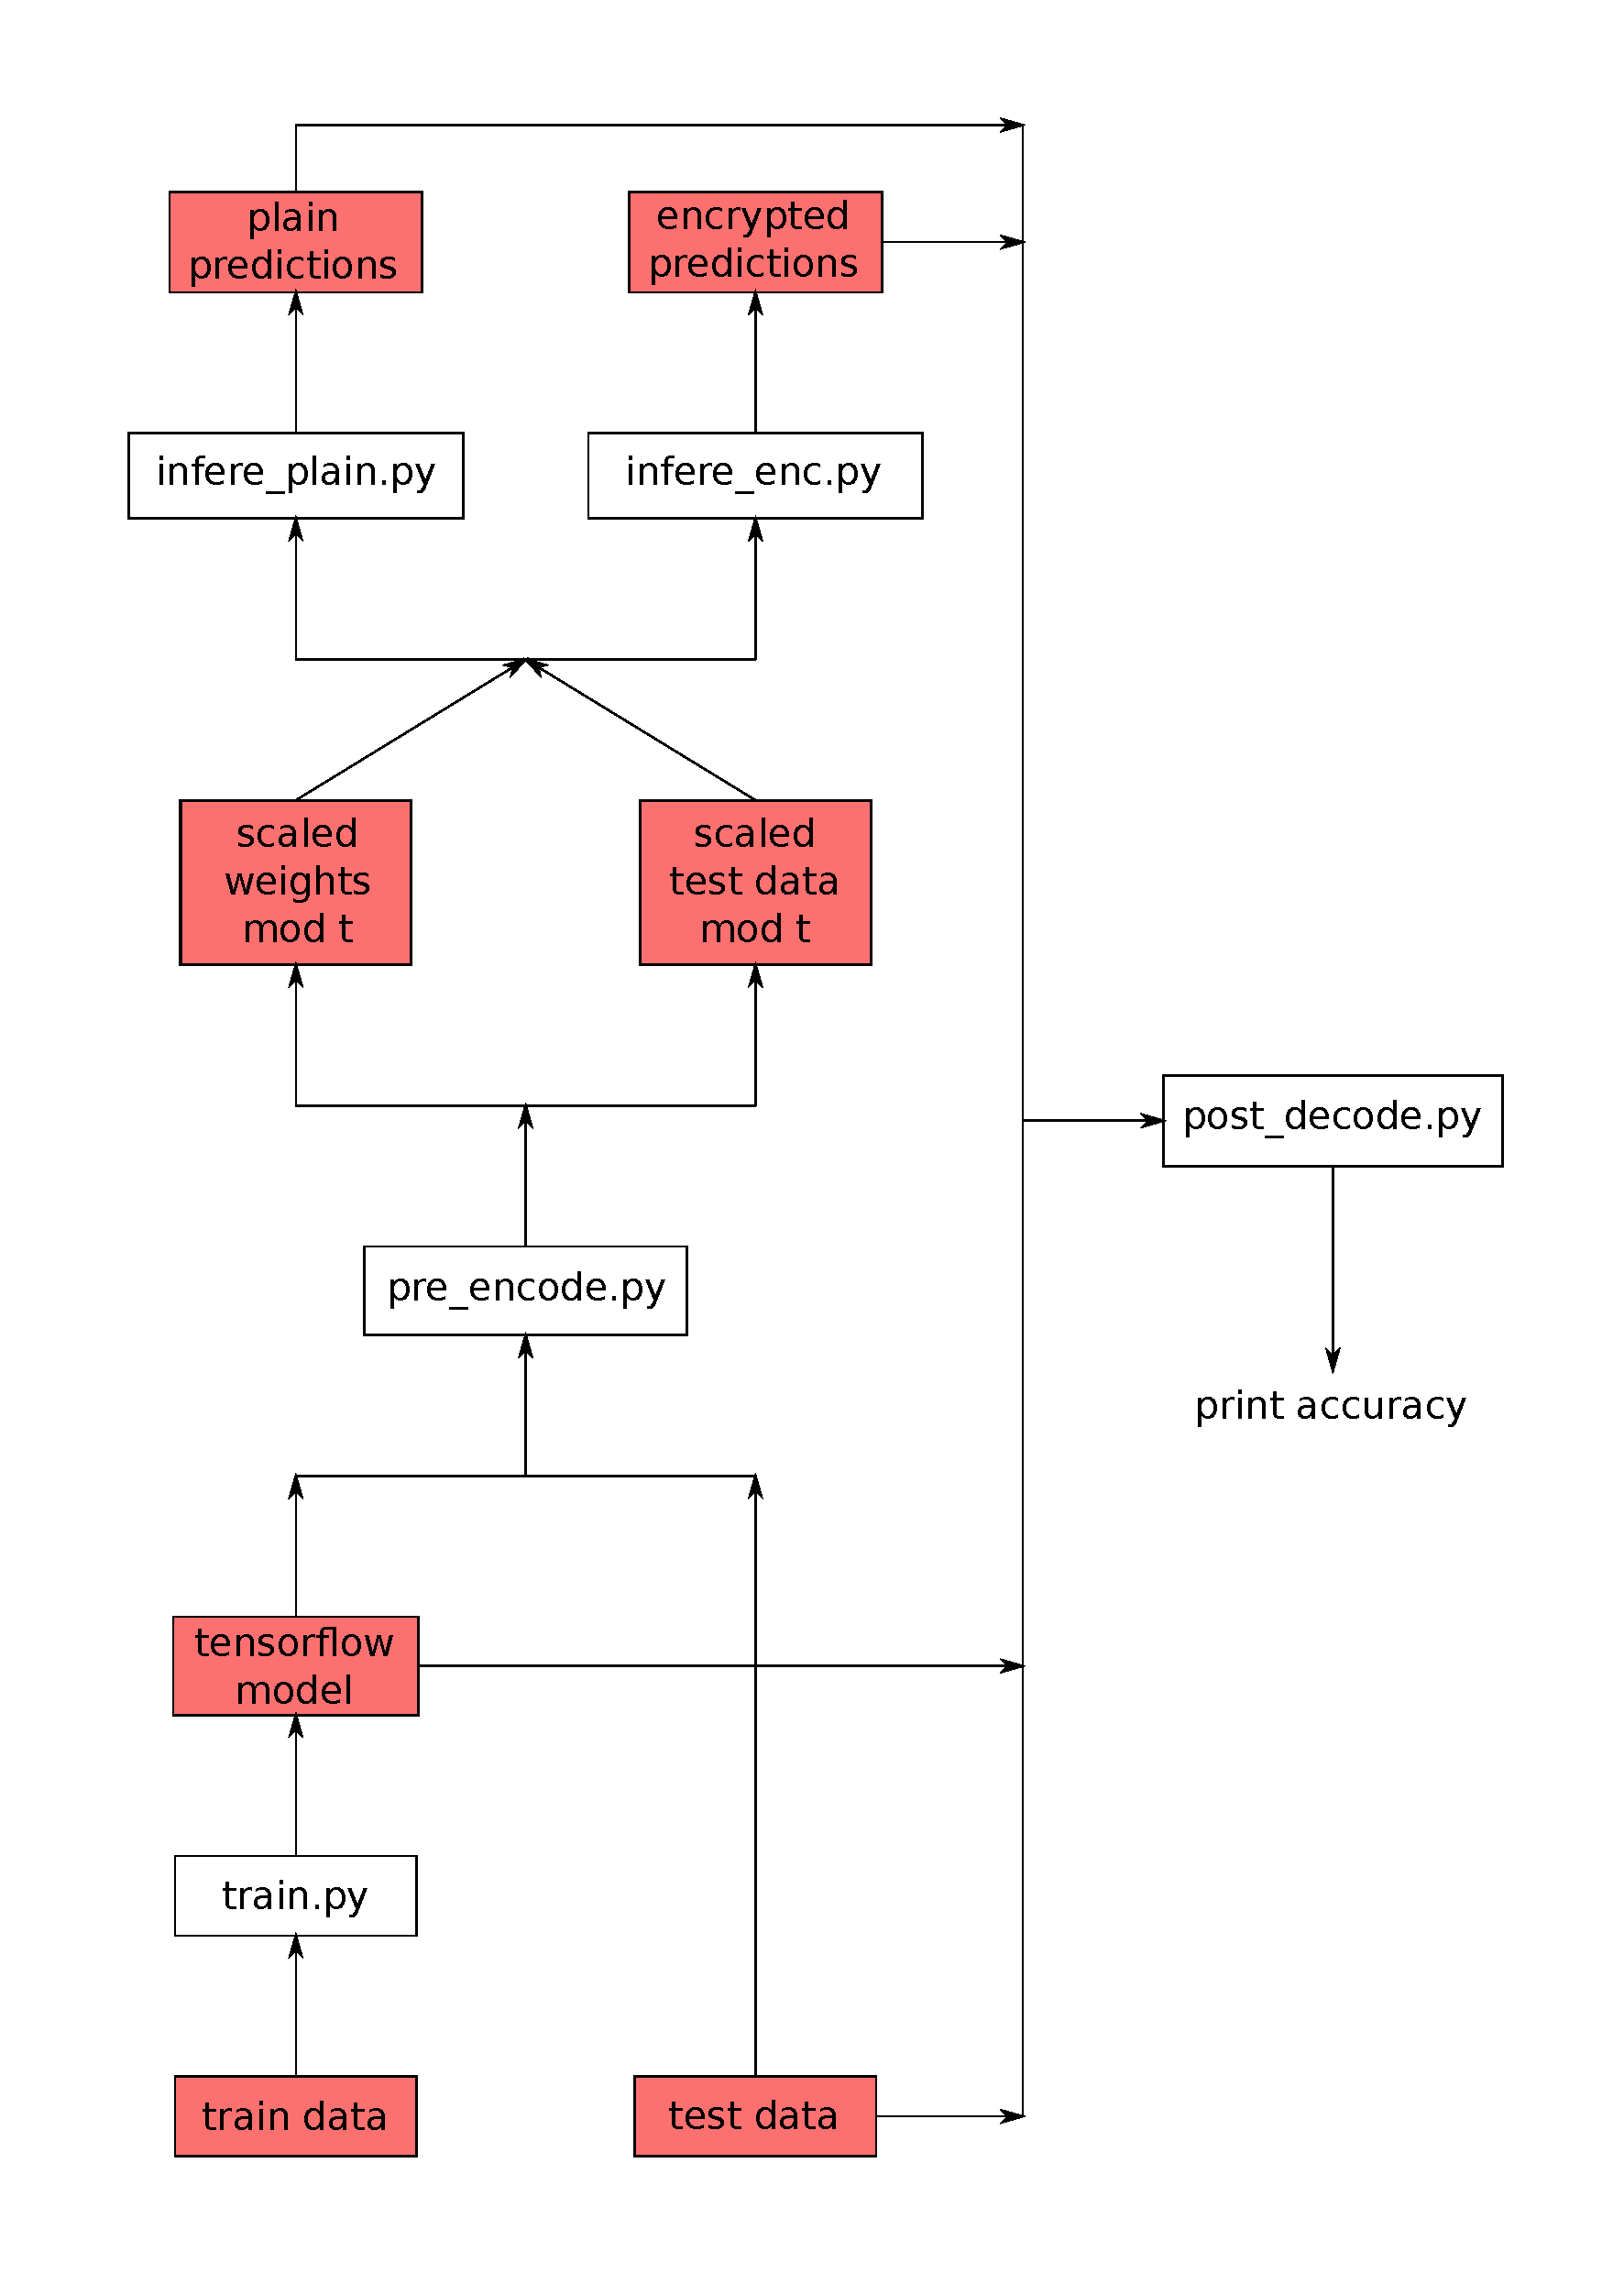
\includegraphics[width=0.9\textwidth]{images/fig4a.pdf}
    \caption{The flow scheme of data between the scripts.}
    \label{fig:im4}
\end{figure}

\subsection{\texttt{train.py}}

As you can see from the diagram, the first script to be executed is \texttt{train.py}. It uses 55000 images and labels from the MNIST database to train a neural network, thanks to the TensorFlow library. The only operations used are sum and product. The network is described in detail in the Section3: Neural network.

\subsection{\texttt{pre_encode.py}}

When executed, this file loads in memory the TensorFlow model generated by \texttt{train.py} from the \texttt{nn_data} folder and applies, on the model as well as on the dataset test, the pre-encoding phase: it multiplies each value by a constant called precision, and performs the reduction modulo $t_i$, with $i = 0,1,2,3,4$. Thus obtains 5 numbers in output for each input number, ie five times the size of the input tensor. The image data and the weights of the neural network thus obtained are saved, respectively, in the \texttt{output_data} folder (with the name of \texttt{plain_layer_0.npy}) and in the \texttt{nn_data} folder.

\subsection{\texttt{infere_plain.py}}

Unlike the other files, \texttt{infere_plain.py} is not strictly necessary for the execution of the project. In fact it was initially developed during the testing and debugging phase of the CryptoNets, but, because it has an intermediate model between the final neural network and the base model calculated with tensorflow, it is useful in order to understand the project. After loading weights and input data into memory, the remaining part of the code is divided into 5 parts, corresponding to the 5 layers of the network. After each layer, it saves the output tensor in the \texttt{output_data} folder (this operation was very useful during the debugging phase). The first layer, the most complicated one, is the convolution layer: for each of the five filters in the map_count, it shifts the filter on the input images, performs a multiplication element-wise, and sums all the values obtained, together to the bias. The resulting sum is reduced modulo $t_i$, and the result is saved in a new output tensor. The indexes of the input and output tensors works in such a way that each image is flattened after the computation. Layers 2 and 4 are identical, and perform the element-wise square operation. Layers 3 and 5 instead correspond to two fully connected layers and take advantage of the NumPy operator .dot() to perform this calculation.

\subsection{\texttt{infere_enc.py}}

\texttt{infere_enc.py} works like \texttt{infere_plain.py}, with the difference that the input data is first encoded and then encrypted. The data are saved after the application of each layer. Moreover, they are saved two more times: once at the beginning, after the encoding and encryption phase, and once at the end, after having executed the inverse procedure. The main difference consists instead in how the input examples are managed: in \texttt{infere_plain.py} the data could and had to be managed separately, but not here. In \texttt{infere_enc.py}, since the data has been encoded in polynomial arrays, the data must be taken in blocks of $(n+1)\cdot\text{q_size}\cdot2$, ie each polynomial must be considered as a single object. Therefore, the index that ran through the images in \texttt{infere_plain.py} becomes four nested for: one to scroll through the blocks of the encrypted messages, one to scroll on the elements of each array, one to scroll on the dividers $q_i$, and one to scroll through the coefficients of each polynomial:

\lstset{frame=tb,
  language=Python,
  breaklines=true,
  showstringspaces=false,
  columns=flexible,
  numbers=left,
  commentstyle=\color{dkgreen},
  stringstyle=\color{mauve},
  tabsize=3
}
\begin{lstlisting}[frame=single]
for poly_group_index in range(poly_groups_count):
  for s_index in range(2):
    for q_index in range(q_size):
      for n_index in range(n_parm+1):
        axis0_index = n_index + (q_index*(n_parm+1)) + (s_index*q_size*(n_parm+1)) + (poly_group_index*enc_poly_size)
        ...
\end{lstlisting}

We added also a print function between lines 3 and 4 which indicates the percentage of progress made for this layer. Layers 3 and 5 work as in the case of \texttt{infere_plain.py}, ie use the NumPy .dot() operator. But in this case, the tensor dtype can no longer be np.uint64, but must be of the object type. This is due to the fact that the data in question are reduced modulo $q_i$, while the weights are reduced modulo $t_i$. This means that while the network weights can reach a maximum of 18 bits (unsigned), the input data values are at most 60 bits. During the multiplication between weights and data the values are therefore 78 bits long, before they're reduced modulo $q_i$ and brought back so into the 60 bit limit. If you force a tensor this way, NumPy automatically transforms the output dtype from np.uint64 to np.float64: the 52 bits of mantissa of the np.float64 type are therefore not enough to contain the entire 78-bit information (before it is reduced with the modulo operation), and there is therefore a loss of precision. This would not be much of a problem if we were operating in the plain data space, but since they are encrypted messages, the loss of precision prevents the FV algorithm from correctly reconstructing the output, resulting in a gibberish output. To prevent this from happening, the tensor must then be forced to use the integer type of Python; in fact it has native support for integers greater than the size of a register (64 bits). In order to accomplish this, we created a function called to_object_dtype() that does just that. After performing multiplication with the .dot() operator, we perform the reduction modulo $q_i$, and finally we add the bias multiplied by the scaling factor $k$ (and reduced again modulo $q_i$). Layers 2 and 4 perform squaring using the function inside the SEAL library.

\subsection{\texttt{post_decode.py}}

The files produced by the two types of inference (plain and encrypted) are compared to see if they are equal. If they are the same, it means that the output calculated through \texttt{infere_enc.py} is correct in the sense that it performed operations on encrypted data in the same way that operations were performed from the file \texttt{infere_plain.py}. In fact, the loss of accuracy in the transition between the model with plain integers and the model with integers but encrypted is and must be zero. The only factor that contributes to the loss of accuracy is in fact the use of integers instead of the original model with real numbers. After comparing the two input files, assuming they are equal, it reconstructs the output using the inverse operation of the crt. It calculates predictions with the argmax() function and also calculates predictions using the original model with real numbers. Finally it prints the accuracy of these two models to compare them.


\section{Results}

We started with a TensorFlow model of 98.43\% accuracy. Using the techniques described in this document together with the cryptographic algorithm the accuracy achieved was 98.40\%, ie only 0.03\% less than the base model. But the processing times were long, longer than those obtained in the original paper. To run tests on a set of 10,000 images, we spent 6 hours on a PC with a single Intel Core i7-4820K CPU running at 3.7GHz, with 12GB of RAM, running the Ubuntu 18.04 operating system. Of these 6 hours, 4 are used by the first layer only. But the time is to be divided between the phases of encoding, encrypting and the application of the neural network. The decoding and decrypting phases turned out to be very fast. Applying the network allows making chunks of 4096 predictions simultaneously, so the actual time taken by an image to be encoded, encrypted and transformed into prediction is less than 2 seconds. A speed equal to about 2048 predictions per hour has thus been obtained. Ie, about one eighth of the speed obtained in \cite{dowlin2016cryptonets}: in the original project 10000 instances are classified in 2263.5 seconds, that is, they reached a speed equal to 15904.6 predictions per hour. The fact that our speed is an eighth of theirs by using a PC with similar characteristics is no coincidence, and should not surprise. In that project, the algorithm used is YASHE, in which a polynomial in $R^n_t$ is transformed into a single polynomial in $R^n_q$. In our case instead, due to the new version of the SEAL library, a polynomial in $R^n_t$ is transformed into an array of polynomials in $R^{n+1}_q$, where the array has two elements, and each element is a set of four polynomials, one for each $q_i$, for a total of 8 polynomials of degree $n+1$. The size of the data to be processed is therefore eight times higher. However, it should be noted that each coefficient of the encrypted message in our case is a 64-bit unsigned variable, while in the original CriptoNets project it is 192 bits. Our algorithm should therefore be three times faster than what we actually got. This did not happen probably due to some differents such as the particular specifics in the PC used. But mostly due to the programming language chosen: the original project was in fact written entirely in the C++ programming language, while we chose to use Python for ease of use. Moreover, part of the time spent was used to save the tensor outputs after each layer and, since the tensors can be very large, this process takes time. The files obtained are in fact very large, and for this reason they have not been uploaded to github:

\begin{center}
\begin{tabular}{ |c|c|c| } 
\hline
File name & Tensor size & File size \\
\hline
\hline
\texttt{enc_layer_0.npy} & (98328, 29, 29, 5) & 3,308 MB \\
\texttt{enc_layer_1.npy} & (98328, 845, 5) & 3,323 MB \\
\texttt{enc_layer_2.npy} & (98328, 845, 5) & 3,323 MB \\
\texttt{enc_layer_3.npy} & (98328, 100, 5) & 466 MB \\
\texttt{enc_layer_4.npy} & (98328, 100, 5) & 393 MB \\
\texttt{enc_layer_5.npy} & (98328, 10, 5) & 47 MB \\
\hline
\end{tabular}
\end{center}

Finally, we need to consider the to_object_dtype() function which, as we found, although necessary for using the NumPy .dot() operator, it also require quite some time. To conclude, we highlight the size of the messages. The messages to be exchanged between the data owner and the cloud for a single chunk of 4096 images are therefore 1103 MB (for the images) and 16 MB (for the predictions).

\begin{figure}[H]
	\centering
	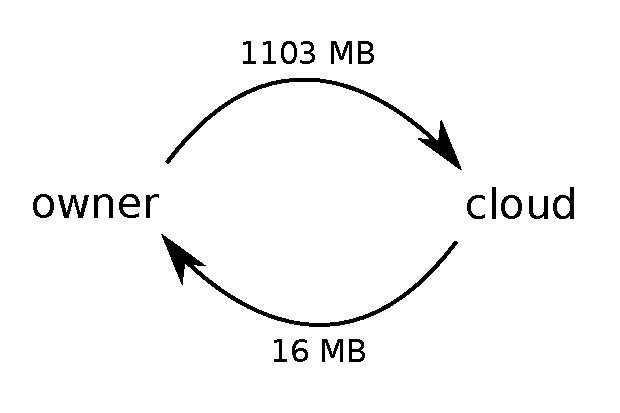
\includegraphics[width=0.5\textwidth]{images/fig5.pdf}
    \caption{Messages exchanged between the owner and the cloud.}
    \label{fig:im4}
\end{figure}


\section{Conclusion}

In recent times global awareness of the importance of data privacy has grown. The IT companies are reviewing their policies regarding data management and improper use that can be made of them. At the same time, however, the great development we have seen in the field of machine learning was made possible also by the free participation, thanks to the presence of free datasets. Moreover some companies could benefit from the use of cloud computing services to obtain predictions on the data they own, but at the same time they do not want to give away the same data. In this project we have followed [paper], and we have shown how it is possible to formulate a neural network that obtains encrypted predictions starting from input data which are also encrypted, thanks to the use of homomorphic algorithms. We focused on the problems arising from the use of this technology and on how to solve them. Moreover we have seen how the use of the v2.3 version of the SEAL cryptography library leads to a notable slow down in the speed of the algorithm compared to the previous versions, up to 8 times slower. This, however, only in relation to the time of execution: we do not have the necessary skills to comment on the safety of the FV algorithm compared to that used in the previous version, namely the YASHE algorithm, for which the judgment on this topic is suspended, but it is important to note that the choice of the cryptographic scheme also has repercussions on security. The advantage of using this version of SEAL, however, is given by the fact that the numbers that are managed are all with a maximum size of 60 bits, that is they can fit entirely in a register, while in the previous version the values were 192 bits. Although it has not been implemented in our project, this allows an easier implementation of an algorithm that exploits the potential of the GPUs.
\clearpage

\bibliography{bibliography}
\bibliographystyle{ieeetr}

\end{document}
